%% ma: L11-B14-0013
%% lop: 11
%% chuong: 4
%% bai: 14
%% dang: 11.14.4
%% loai: TN4
%% muc: TH
%% dap_an: "D"
%% nguon: "tai-lieu-hoc-tap-mon-toan-lop-11-theo-chuong-trinh-giao-duc-pho-thong-2018.pdf (Lớp Toán Thầy Duy, Phạm Lê Duy, THPT Chu Văn An), Chương 4 Bài 5, Phần 1, Câu 8 (tr.528)"
%% kien_thuc: "Lớp 11 Bài 14 (phép chiếu song song)"
%% trang_thai: chinh-thuc
%% ghi_chu: "Hình TikZ dựng lại theo hình gốc (vị trí điểm xấp xỉ). Đã duyệt 03/11/2026."
\begin{ex}
Trên hình bên, ta có phép chiếu song song theo phương $d$ và mặt phẳng chiếu $(P)$; $AB\parallel CG$ và $AB=DG$; $A^{\prime},B^{\prime},C^{\prime},D^{\prime},E^{\prime},G^{\prime}$ lần lượt là hình chiếu của $A,B,C,D,E,G$ qua phép chiếu nói trên. Khi đó, có bao nhiêu khẳng định đúng trong các mệnh đề sau (i) $\dfrac{DG}{AB}=\dfrac{D^{\prime}G^{\prime}}{A^{\prime}B^{\prime}}=1$. (ii) $\dfrac{C^{\prime}D^{\prime}}{D^{\prime}E^{\prime}}=\dfrac{CD}{DE}$. (iii) $D^{\prime}G^{\prime}=A^{\prime}B^{\prime}$.
\begin{center}
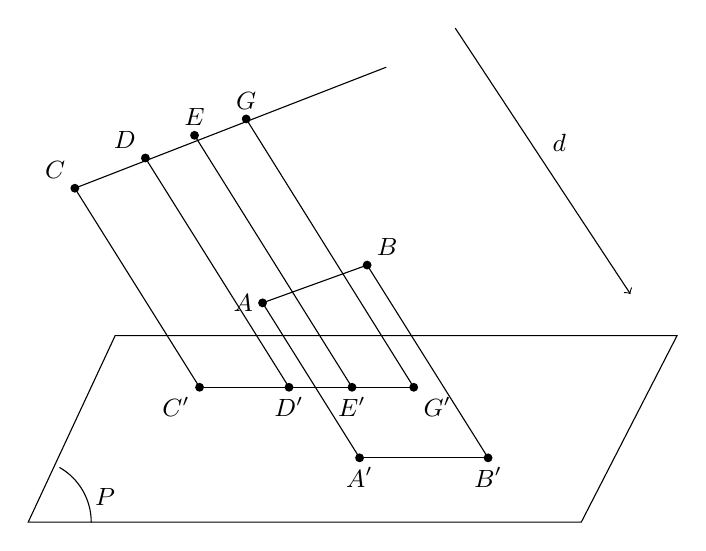
\begin{tikzpicture}[scale=1.6,line cap=round,font=\small]
\draw (0.63,0)--(5.09,0)--(4.33,-1.48)--(-0.06,-1.48)--cycle;
\draw (-0.06,-1.48) ++(0.5,0) arc (0:60:0.5);
\node at (0.55,-1.28){$P$};
\draw (0.31,1.17)--(2.78,2.13);
\draw (0.31,1.17)--(1.30,-0.41); \fill (0.31,1.17) circle(1pt) node[above left]{$C$}; \fill (1.30,-0.41) circle(1pt) node[below left]{$C^{\prime}$};
\draw (0.87,1.41)--(2.01,-0.41); \fill (0.87,1.41) circle(1pt) node[above left]{$D$}; \fill (2.01,-0.41) circle(1pt) node[below]{$D^{\prime}$};
\draw (1.26,1.59)--(2.51,-0.41); \fill (1.26,1.59) circle(1pt) node[above]{$E$}; \fill (2.51,-0.41) circle(1pt) node[below]{$E^{\prime}$};
\draw (1.67,1.72)--(3.00,-0.41); \fill (1.67,1.72) circle(1pt) node[above]{$G$}; \fill (3.00,-0.41) circle(1pt) node[below right]{$G^{\prime}$};
\draw (1.80,0.26)--(2.63,0.56); \fill (1.80,0.26) circle(1pt) node[left]{$A$}; \fill (2.63,0.56) circle(1pt) node[above right]{$B$};
\draw (1.80,0.26)--(2.57,-0.97); \draw (2.63,0.56)--(3.59,-0.97); \fill (2.57,-0.97) circle(1pt) node[below]{$A^{\prime}$}; \fill (3.59,-0.97) circle(1pt) node[below]{$B^{\prime}$};
\draw (2.57,-0.97)--(3.59,-0.97);
\draw (1.30,-0.41)--(3.00,-0.41);
\draw[->] (3.33,2.44)--(4.72,0.33) node[midway,above right]{$d$};
\end{tikzpicture}
\end{center}
\choice{$0$.}{$1$.}{$2$.}{\True $3$.}
\loigiai{\sloppy Phép chiếu song song bảo toàn tỉ số độ dài của hai đoạn thẳng nằm trên hai đường thẳng song song (hoặc cùng nằm trên một đường thẳng). (i) $DG\parallel AB$, $\dfrac{DG}{AB}=1$ nên $\dfrac{D^{\prime}G^{\prime}}{A^{\prime}B^{\prime}}=1$: đúng. (ii) $C,D,E$ thẳng hàng nên $\dfrac{C^{\prime}D^{\prime}}{D^{\prime}E^{\prime}}=\dfrac{CD}{DE}$: đúng. (iii) từ (i), $D^{\prime}G^{\prime}=A^{\prime}B^{\prime}$: đúng. Cả $3$ khẳng định đều đúng.}
\end{ex}
